%%%%%%%%%%%%%%%%%%%%%%%%%%%%%%%%%%%%%%%%%%%%%%%%%%%%%%%%%%%%
% MAL for tekniske rapporter
% her har jeg gjort en endring1
%
% (C) Copyright Ola Jetlund 2025
%     - det er lov å kopiere og gjenbruke denne filen uten
%       å referere til forfatter, originalt filnavn eller noe
%       som helst.
%       her har jeg også gjort en endring2
%
% Alle kommandoer er forklart under.
% Prosent % i starten på en linje angir kommentar.
%%%%%%%%%%%%%%%%%%%%%%%%%%%%%%%%%%%%%%%%%%%%%%%%%%%%%%%%%%%%

%%%%%%%%%%%%%%%%%%%%%%%%%%%%%%%%%%%%%%%%%%%%%%%%%%%%%%%%%%%%
% FØRST setter vi opp dokumentet ved å inkludere pakker som øker
% funksjonaliteten.
%
% Vanlige dokumentklasser er article, report, book, letter etc
% Her er det valgt "report"
% [12pt] angir skriftstørrelse 12pt som er litt stort. Men lesbart.
% [a4paper] angir arkstørrelsen vi kan printe ut på uten skalering.
\documentclass[11pt,a4paper,twocolumn]{article}

% Babel - inneholder en del språkavhengige termer som f.eks.
% datoformat. Ved å legge på
% [norsk]
% får vi automatisk norske ord for disse:
\usepackage[norsk]{babel}

% Geometry - Ikke alle liker standardmargene til LaTeX.
% Denne pakken kan fikse dette. Her er følgende brukt:
% [a4paper] - unødvendig siden det står lenger opp, men gjør ikke noe.
% [top=2cm,bottom=2cm,left=3cm,right=3cm] - angir luft i margene.
% [marginparwidth=1.75cm] er marg som kan inneholde tekst, symboler etc.
% Mer: https://www.overleaf.com/learn/latex/Page_size_and_margins
\usepackage[a4paper,
            top=2cm,
            bottom=2cm,
            left=3cm,
            right=3cm,
            marginparwidth=1.75cm]{geometry}

% amsmath - gir bedre matematiske symboler samt flere muligheter.
\usepackage{amsmath}

% cleveref - For kryssreferanser inne i et dokument
% [norsk] - Kapittel/Figur/Tabell etc.
% Referanser gjøres ved å legge en "label" nederst i figur, tabell, ligning
% slik at vi i teksten kan referere med "cref"
% \label{fig:et-bilde} kan da refereres til med \cref{fig:et-bilde}
\usepackage[norsk]{cleveref}

% enumitem - LaTeX lager kulepunkter og numrerte lister med
%   \begin{itemize}
%       \item Ett kulepunkt
%       \item Et til...
%   \end{itemize}
%   \begin{enumerate}
%       \item Her får vi 1. og litt tekst
%       \item Her får vi 2. og litt tekst
%   \end{enumerate}
% Pakken enumitem gir oss mulighet til å gjøre disse litt annerledes:
%  F.eks.:
%       \begin{enumerate}[a)]
%            \item Gir oss punkter med a), b), c) etc.
%       \end{enumerate}
\usepackage[shortlabels]{enumitem}

% graphics - gir oss \includegraphics for å inkludere bilder:
% F.eks.:
%       \includegraphics[width=0.3\textwidth]{mittbilde.jpg}
\usepackage{graphicx}

% fontenc - for å sørge for gode fonter - helt unødvendig på Overleaf.
\usepackage[T1]{fontenc}

% url - for å skrive nettadresser
% F.eks.:
%   \url{vg.no}
\usepackage[hyphens]{url}

% lipsum - Gir oss en blindtekst å leke med når vi ikke har noe fornuftig å skrive ...
\usepackage{lipsum} 

% siunitx - handler egentlig om enheter, men også om
% formatering av tall.
% sisetup{} - gjør at vi kan sette en del parametre:
%  I eksemplet under får vi j for komplekse tall og ikke i.
%  Vi får 2,3 og ikke 2.3 fordi decimal-marker settes til ,
%
% Nå kan vi skrive et tall med enhet som f.eks.
%   \qty{200}{\ohm}
% og et tall som
%   \num{2,1828}
% og få alt formatert riktig uansett om vi er i
% matematikk eller tekst.
\usepackage{siunitx}
\sisetup{
  output-complex-root = \ensuremath{\mathit{j}},
  complex-root-position = before-number,
  exponent-product = \cdot,
  output-decimal-marker = {,}
}

% Det er ikke med tikZ og circuitikZ jeg lager mine kretser,
% men med et lignende system, så la oss laste inn disse også:
\usepackage{tikz}
\usepackage{circuitikz}
\usetikzlibrary{arrows.meta,positioning,calc}

% pgfplots - Jeg plotter mine kurver direkte i LaTeX.
% Eksempel lenger ned i fila.
% compat=1.18 har med versjoner å gjøre og er bare der for at Overleaf
% ikke skal klage så mye.
\usepackage{pgfplots}
\pgfplotsset{compat=1.18}

% Jeg liker ikke at et avsnitt starter med innrykk.
% Kan fjernes for de som liker sånt.
\setlength{\parindent}{0pt}

%%%%%%%%%%%%%%%%%%%%%%%%%%%%%%%%%%%%%%%%%%%%%%%%%%%%%%%%%%%%
% START HER!
%%%%%%%%%%%%%%%%%%%%%%%%%%%%%%%%%%%%%%%%%%%%%%%%%%%%%%%%%%%%
\title{Rapportskriving i ELI1300}
\author{Ola Jetlund\\Gruppe DrOJ}
\date{17.05.2026} 

\urldef{\myoverleafurl}\url{https://tinyurl.com/2yfbtdez}
\begin{document}
\maketitle % Setter sammen \title og \author og \date

%%%%%%%%%%%%%%%%%%%%%%%%%%%%%%%%%%%%%%%%%%%%%%%%%%%%%%%%%%%%
% Abstract eller sammendrag:
\begin{abstract}
    Denne rapporten oppsummerer det praktiske arbeidet med analyse, bygging og vurdering av elektriske kretser gitt i øvingsoppgavene. Arbeidet omfatter både teoretiske beregninger og eksperimentelle målinger, med fokus på metode, resultater og refleksjon rundt gjennomføringen.    
\end{abstract}

%%%%%%%%%%%%%%%%%%%%%%%%%%%%%%%%%%%%%%%%%%%%%%%%%%%%%%%%%%%%
% Innholdsfortegnelse automatisk generert:
%\tableofcontents
% Her er den kommentert ut siden dette er en kortkort rapport!

%%%%%%%%%%%%%%%%%%%%%%%%%%%%%%%%%%%%%%%%%%%%%%%%%%%%%%%%%%%%
% Nytt kapittel 
% Siden jeg bruker "article" er det ingen chapter slik som i 
% "book" eller "report"
% Nivåer: chapter, section, subsection
%%%%%%%%%%%%%%%%%%%%%%%%%%%%%%%%%%%%%%%%%%%%%%%%%%%%%%%%%%%%
% Nytt avsnitt
\section{Innledning}
Rapporter som leveres i ELI1300 skal skrives i \LaTeX. Dette gjøres enklest på nettstedet
Overleaf: \url{www.overleaf.com}.
\subsection{Hensikt}
Hensikten med denne rapporten er å gi en innføring i rapportskriving generelt og i bruk av \LaTeX. Alle delene som inngår her, skal være med i alle tekniske rapporter. Det er viktig med tydelig oppdeling i kapitler. Bruk av tabeller, figurer og referanser er avgjørende for å produsere en rapport som kan godkjennes.

Denne eksempelrapporten med kommentarer som forklarer koden er gjort tilgjengelig i fotnoten\footnote{\myoverleafurl}.


%%%%%%%%%%%%%%%%%%%%%%%%%%%%%%%%%%%%%%%%%%%%%%%%%%%%%%%%%%%%
% Nytt delavsnitt 
\subsection{Utstyrsliste}

Utstyrsliste kan plasseres enten i innledningen eller under praktisk arbeid, avhengig av hva som passer best for rapporten.

Listen bør inneholde typebetegnelse, fabrikat og eventuelt nummerering dersom det benyttes utstyr som er nummerert av laboratorieansvarlig.

% En sentrert tabell med tittel over og label for 
% kryssreferanse:
\begin{table}[ht] %[h] for å plassere den så nær "her" som mulig.
    \centering
    % Caption - gir overskriften
    \caption{Utstyrsliste}
    % Label så vi senere kan skrive \cref{tab:utstyr} for å
    % referere til tabellen i teksten vår.
    \label{tab:utstyr}
    % {|l|l|l|} er tre kolonner med tekst venstrejustert
    % og med vertikale streker for å skille kolonner
    \begin{tabular}{|l|l|l|}\hline %\hline = horisontal strek
        Utstyr      & Type           & Fabrikat   \\\hline\hline
        NMOS        & IRLB8748PBF    &Infineon  \\
        Multimeter  & Digitalt       &FLUKE \\
        Batteri     & \qty{9}{\volt} & IKEA \\
        Motstand    & \qty{200}{\ohm}&- \\\hline 
    \end{tabular}
\end{table}


%%%%%%%%%%%%%%%%%%%%%%%%%%%%%%%%%%%%%%%%%%%%%%%%%%%%%%%%%%%%
% Nytt avsnitt
\subsection{Krav til rapporter og gode råd}
Det er ikke mange krav til rapportene, men de skal følges. Disse er gitt i \cref{app:krav}. I \cref{app:god} er det gitt noen gode råd.





%%%%%%%%%%%%%%%%%%%%%%%%%%%%%%%%%%%%%%%%%%%%%%%%%%%%%%%%%%%%
% Nytt kapittel
\section{Teoretisk del}

%%%%%%%%%%%%%%%%%%%%%%%%%%%%%%%%%%%%%%%%%%%%%%%%%%%%%%%%%%%%
% Nytt avsnitt
\subsection{Oppgave X}

%%%%%%%%%%%%%%%%%%%%%%%%%%%%%%%%%%%%%%%%%%%%%%%%%%%%%%%%%%%%
% Setter inn et bilde - kommenteres ut om bildet ikke finnes
%
% includegraphics forstår pdf, png, jpg osv.
\begin{figure}[ht]
\centering 

\includegraphics[width=0.5\linewidth]{lion.png}
\caption{\TeX-løven.}
\label{fig:olabilde}
\end{figure}

Alle figurer og bilder som inkluderes i rapporten skal omtales og refereres til i teksten, for eksempel med \cref{fig:olabilde}. Dersom bildet mangler, må linjen for å inkludere det fjernes fra kommentering og erstattes med riktig filnavn når bildet er tilgjengelig.

Matematisk notasjon og formler bør presenteres tydelig og korrekt. For mer informasjon om matematikk i \LaTeX, anbefales det å lese \cite{Oetiker2007}.

\begin{enumerate}[a)]
    \item Matematikk kan presenteres direkte i teksten, for eksempel $x= \frac{-b \pm \sqrt{b^2 - 4ac}}{2a}$.
    \item Det er også mulig å sette opp formler på egen linje uten referanse:
    \[
        x= \frac{-b \pm \sqrt{b^2 - 4ac}}{2a}
    \]
    \item For formler som skal refereres til senere, bør ligningsnummer benyttes:
    \begin{equation}
        x= \frac{-b \pm \sqrt{b^2 - 4ac}}{2a}
        \label{eq:kv_lf}
    \end{equation}
    \item Det er da mulig å referere til ligningen over med \cref{eq:kv_lf} eller \Cref{eq:kv_lf}.
\end{enumerate}

%%%%%%%%%%%%%%%%%%%%%%%%%%%%%%%%%%%%%%%%%%%%%%%%%%%%%%%%%%%%
% Nytt kapittel
\section{Praktisk arbeid}
For rapporter i dette emnet skal det under praktisk arbeid være tegnet opp for eksempel hvordan kretsen er koblet opp på breadboard. Og hvordan kretsene er målt. En kretstegning slik som i \cref{fig:circ_diode} er naturlig å ha med her.
%%%%%%%%%%%%%%%%%%%%%%%%%%%%%%%%%%%%%%%%%%%%%%%%%%%%%%%%%%%%
% For the love of all those who asked: A circuit
\begin{figure}
    \centering
    \begin{circuitikz}[american]
        \draw (0,0) to [V,l={$v_s=\qty{9}{\volt}$},invert] (0,2);
        \draw (0,2) to[R, l=\qty{220}{\ohm},european] (2,2);
        \draw (2,2) to[/tikz/circuitikz/bipoles/length=1cm,led] (2,0);
        \draw (0,0) -- (2,0);
    \end{circuitikz}
    \caption{Diodekretsen fra introkurset tegnet med CircuitTikZ.}
    \label{fig:circ_diode}
\end{figure}
%%%%%%%%%%%%%%%%%%%%%%%%%%%%%%%%%%%%%%%%%%%%%%%%%%%%%%%%%%%%


%%%%%%%%%%%%%%%%%%%%%%%%%%%%%%%%%%%%%%%%%%%%%%%%%%%%%%%%%%%%
% Nytt kapittel
\section{Resultater}
%%%%%%%%%%%%%%%%%%%%%%%%%%%%%%%%%%%%%%%%%%%%%%%%%%%%%%%%%%%%
% Nytt avsnitt
\subsection{Et plott}
Plot kan genereres direkte i \LaTeX{} ved hjelp av pakkene \verb|tikZ| og \verb|pgfplots|, som er inkludert i starten av denne filen. Begge pakkene har omfattende og god dokumentasjon.
%%%%%%%%%%%%%%%%%%%%%%%%%%%%%%%%%%%%%%%%%%%%%%%%%%%%%%%%%%%%
% Plot - start
% 
% TILPASS alle stedene under hvor det står YYY
\begin{figure}[htb] %htbn står for: "prøv å plassere figuren Here, or Top or Bottom  - in that order."
\centering
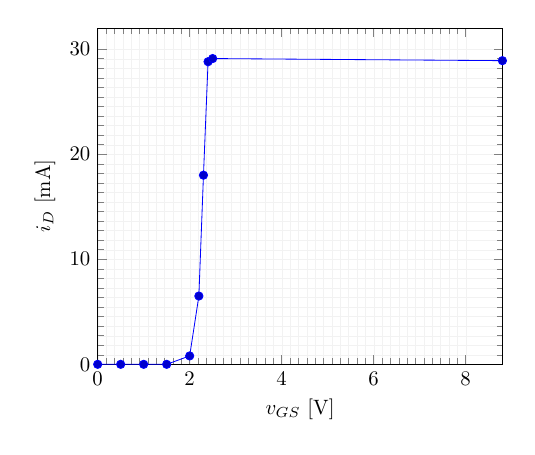
\begin{tikzpicture}[scale=.75]
  \begin{axis}[
  ylabel=\(i_{D}~\text{[mA]}\), % YYY
  xlabel=\(v_{GS}~\text{[V]}\), % YYY
  grid=both,
  grid style={line width=.1pt, draw=gray!10},
  minor tick num=10,
  xmin = 0,    % YYY
  xmax = 8.8,  % YYY
  ymin=0,      % YYY 
  ymax=32]     % YYY
\addplot coordinates {
(0.0,   0)  % YYY
(0.5,   0)  % YYY
(1.0,   0)  % YYY
(1.5,   0)  % YYY
(2.0, 0.8)  % YYY
(2.2, 6.5)  % YYY
(2.3,18.0)  % YYY
(2.4,28.8)  % YYY
(2.5,29.1)  % YYY
(8.8,28.9)  % YYY
};
\end{axis}
\end{tikzpicture}
\caption{Mitt plott - gjenbruk meg gjerne.}
\label{fig:plot}
\end{figure}



%%%%%%%%%%%%%%%%%%%%%%%%%%%%%%%%%%%%%%%%%%%%%%%%%%%%%%%%%%%%
% Diskusjon - start
\section{Diskusjon}

Diskusjonsdelen skal inneholde vurderinger og refleksjoner rundt resultatene. Her kan det diskuteres feilkilder, usikkerhet, alternative løsninger og hvordan resultatene stemmer overens med teori og forventninger.


\section{Konklusjon}

Konklusjonen kan være et eget kapittel eller inngå som en del av diskusjonen, avhengig av rapportens omfang. En god konklusjon oppsummerer hovedfunnene og trekker frem sentrale erfaringer og læringspunkter fra arbeidet.


I ELPE1300 skal konklusjonen inneholde et refleksjonsnotat om gjennomføringen av øvingen, inkludert erfaringer, nytteverdi og læringsutbytte.



\begin{thebibliography}{9}
\bibitem{texbook}
Donald E. Knuth (1986) \emph{The \TeX{} Book}, Addison-Wesley Professional.

\bibitem{lamport94}
Leslie Lamport (1994) \emph{\LaTeX: a document preparation system}, Addison
Wesley, Massachusetts, 2nd ed.

\bibitem{Oetiker2007}
{Oetiker, Tobias and Partl, Hubert and Hyna, Irene and Schlegl, Elisabeth} (2007), \url{http://tobi.oetiker.ch/lshort/lshort.pdf}

\end{thebibliography}

\newpage
\appendix
\section{Krav til rapportene}\label{app:krav}
Det er ikke mange krav til rapportene, men ting skal settes opp skikkelig:
\subsection{Tydelig informasjon}
På første side skal det stå
  \begin{itemize}
    \item tittel på rapporten
    \item navn på forfattere - fulle navn
  \end{itemize} 
\subsection{Nummerering}
Alle \textbf{formler}, \textbf{figurer} og \textbf{tabeller} skal nummereres og refereres til i tekst.
\begin{itemize}
  \item Alle figurer og tabeller skal ha caption.
  \item Figurer har caption under, tabeller har caption over.
\end{itemize}
\subsection{Format og lengde}
\begin{itemize}
  \item Enspalte eller tospalte.
  \item Maksimalt antall sider er 5.
  \item Rapporten skal leveres som PDF.
  \item Rapporten skal skrives i \LaTeX
\end{itemize} 

\subsection{Språk i tekniske rapporter}
Tekniske rapporter skal ha et formelt og presist språk. Unngå personlig tiltale og bruk av pronomen som "vi", "jeg", "du", "han", "hun", "dere", "deg", samt forkortelser som "etc.", "osv." og "f.eks.". Rapporten skal fokusere på det faglige innholdet, ikke på forfatter eller gruppe.

Det anbefales å bruke rettskrivingsverktøy eller KI for å sikre korrekt språk.

\subsection{Symboler}
Symbolbruk skal være riktig. For eksempel:
  \begin{itemize}
    \item $v$ for spenning. Ikke $U$.
    \item små bokstaver for størrelser som kan variere slik som strøm og spenning. Store bokstaver for størrelser som er konstante slik som resistans og kapasitans.
    \item Bruk subscript for å skille mellom forskjellige elementer. For eksempel $v_a$ og $v_b$ for spenning over to forskjellige elementer.
    \item Brukt standardiserte enheter. For eksempel \qty{1}{\volt} og \qty{1}{\ampere}. Ikke $1V$ og $1A$. Det vil si bruk:
    \begin{verbatim}
      \qty{1}{\ampere}
    \end{verbatim}
    Og ikke:
    \begin{verbatim}
      1A og $1A$
    \end{verbatim}
  \end{itemize}

\subsubsection{Innhold og oppdeling}
\small %Litt mindre font for denne listen
En teknisk rapport bør inneholde følgende elementer:
\begin{enumerate}[1)]
    \item[*] Sammendrag (ofte ikke nummerert)
    \item Innledning
    \item Teoretisk del
    \item Praktisk arbeid
    \item Målinger eller Resultater
    \item Diskusjon
    \item Konklusjon
    \item[*] Bibliografi eller Referanser (ofte ikke nummerert)
\end{enumerate}
\normalsize % tilbake til normal fontstørrelse
Det er viktig å holde disse kapitlene adskilt. Resultater skal for eksempel  ikke presenteres under praktisk arbeid.

\section{Gode råd}\label{app:god}
\begin{enumerate}[I]
    \item Rapporten bør være selvstendig, slik at leseren forstår innholdet uten å ha tilgang til oppgaveteksten. Unngå å kopiere oppgaveteksten direkte; beskriv heller oppgavene med egne ord.
    \item Delkapitler som ``Oppgave 1'' MÅ unngås. Skriv heller for eksempel ``Spenningsdeler med last''.
    \item Bruk tid på å lage tydelige og informative figurer. Skannede bilder eller mobilbilder er aldri tillatt..
    \item Vær konsis. En kort, oversiktlig og ryddig rapport som besvarer alle spørsmål er bedre enn en lang rapport med unødvendig tekst.
\end{enumerate}


\end{document}
